\section{引言}
受益于机器学习的蓬勃发展,机器学习提供了强大的工具来处理诸如自然语言处理,数据挖掘,信号处理与识别等诸多领域。尤其在信号处理领域,由于这些机器学习和深度学习新技术的出现,使得以前只有在科幻片里才能见到的科技应用正在一步一步成为现实。
机器学习和信号处理的结合涌现出了大量新奇的技术。例如通过分析脑电波控制机器手臂和机械腿辅助残疾人进行活动;亦或是嘈杂的环境中提取人的声音,或是耳机中的主动降噪都用到了机器学习和信号处理作为核心技术去实现。而这些功能都可以进一步分解成几个子问题:1.对采集的信号进行分析,提取出感兴趣的部分。2.对信号进行滤波,把噪声滤除。3.进一步得到不同的特定模式,并学习区分不同的模式。
所以滤波的好坏在很大程度上会影响到后续各个环节的结果,最终影响到整个应用的性能。支持向量机在二维数据上有出色的性能表现,能够对数据进行拟合回归,故采用SVM作为滤波的核心算法。
\section{相关概念及介绍}
\subsection{支持向量机(SVM)算法}
支持向量机(SVM)分析是一种流行的机器学习工具,常用于分类和回归。SVM是由Vapnik于1995年首次提出的一种新颖的非线性学习方法。SVM具备坚实的理论基础,较好地实现了结构风险最小化原则,这是神经网络等其他机器学习方法不具备的。它通过对凸二次规划问题进行求解, 在有限样本学习能力与模型复杂度之间寻求折中, 以获取最佳泛化性能。图1为SVM体系结构图 \ref{fig:SVM},其中x(i)为输入的自变量特征值,K为核函数,通过核函数将自变量x(i)映射到高维特征空间,在该特征空间进行线性回归[2],得到输出Y。
\begin{figure}[!htbp]
    \centering
    %trim option's parameter order: left bottom right top
    \includegraphics[width=7cm]{pic/svm.png}%trim = 0mm 0mm 0mm 0mm,clip,
    \caption{SVM体系结构。}
    \label{fig:SVM}
\end{figure}

当SVM用于处理回归问题时,目标是找到一个函数f(x),它对每个训练点x偏离$y_n$的值不大于ε,同时尽可能平坦。假设我们有一组训练样本,其中$x_n$是一个包含n个观测值的集合,$y_n$是对应的观测结果。
为了找到线性方程$f(x)=x′β+b$, 确保其足够平坦,需要找到满足最小范数$(β′β)$条件的f(x)。这是一个凸优化问题,以最小化$J(β)=12β′$β。

并满足如下等式:
\begin{equation}
\forall\ n:\left|y_n-\left(x_n^\prime\beta+b\right)\right|\le\varepsilon
\end{equation}

引入松弛变量后推出目标函数,也称为原始公式
\begin{equation}
J\left(\beta\right)=0.5\ast\beta^\prime\beta+C\sum_{n=1}^{N}{\xi_n+\xi_n^\ast}
\end{equation}

约束为:

\begin{equation}
\begin{gathered}
\forall\ n:y_n-\left(x_n^\prime\beta+b\right)\le\varepsilon+\xi_n\\
\forall\ n:\left(x_n^\prime\beta+b\right)-y_n\le\varepsilon+\xi_n^\ast\\
{\forall n:\xi}_n^\ast\geq0\\
\forall\ n:\ \xi_n\geq0
\end{gathered}
\end{equation}

常数C是框约束,是一个正数值,它控制对\varepsilon 边界(\varepsilon )之外的观测值施加的惩罚,并有助于防止过度拟合(正则化)。该值决定了f(x)的平面度与允许大于ε的偏差量之间的权衡,用于寻求泛化性能与训练误差之间的折中。
线性ε-不敏感损失函数将观测值ε距离内的误差视为零而忽略。根据观测值y与ε边界之间的距离来测量误差。用如下的数学公式表示:

\begin{equation}
L_\varepsilon= 
\begin{cases}
0&               \text{if} |y-f(x)|\leq \varepsilon\\
|y-f(x)|-\varepsilon&       \text{otherwise}
\end{cases}
\end{equation}

\subsection{MVDR算法}
在介绍MVDR算法前,先引入相关线性滤波的知识[4]。
x是期望信号,为了得到x,需要对观测信号y进行线性滤波。

\begin{equation}
\begin{aligned}
z&=h^Hy\\
&= h^H\left(x+v_0\right)
&=x_{fd}+v_{rn}
\end{aligned}
\end{equation}

$v_0$是加性白噪声.z是x的估计,也是滤波器的输出信号,

\begin{equation}
h=\left[h_1h_2\ldots h_M\right]^T
\end{equation}

是长度为M的复数滤波器。

\begin{equation}
x_{fd}= h^Hx
\end{equation}

是期望滤波信号
\begin{equation}
v_{rn}=\ h^Hv_0
\end{equation}

是残差噪声。
\begin{equation}
I_M={Q'}_X{Q'}_X^H+{Q''}_X{Q''}_X^H
\end{equation}

${Q'}_X$是$M*R_X$维大小的矩阵,包含$\Phi_X$非零特征值对应的特征向量。
通过(9)可以把期望信号表示如下
\begin{equation}
\begin{aligned}
x&=Q_XQ_X^Hx
&={Q'}_X{Q'}_X^H\ x
\end{aligned}
\end{equation}

并从公式(10)推导出无失真约束
\begin{equation}
h^HQ_x'=i_i^TQ_x'
\end{equation}

\section{算法结合}
将公式(11)进一步推导为符合SVM目标函数的不等式约束
\begin{equation}
h^HQ_x^\le i_i^TQ_x'
\end{equation}

构造拉格朗日方程
\begin{equation}
\begin{aligned}
&J\left(w,\xi,{\xi^\prime}_i,a,a^\prime,\gamma,\gamma^\prime,\beta\right)=0.5||w||^2+C\sum\limits_{i=1}^{n}(\xi_i +\xi'_i)\\
&-\sum_{i=1}^{N}{a_i\left(w^Tx_i+b-d_i+\varepsilon+\xi_i\right)}\\
&-\sum_{i=1}^{N}{a_i\left(d_i-w^Tx_i-b+\varepsilon+{\xi'}_i\right)}\\
&-\sum_{i=1}^{N}{\beta_i\left(-h^HQ_{xi}'+i_i^TQ'\right)}
\end{aligned}
\end{equation}

\section{仿真实验}
为了测试该算法回归性能,在matlab上进行实验验证。设期望信号由五个谐波随机过程组成:$x\left(t\right)=\sum_{k=1}^{5}{A_kcos\left(2\pi f_kt+\phi_k\right)}$,其中振幅$A_k=0.5/k\left(k=1,\ldots,5\right)$,频率$f_k=0.05+0.1\left(k-1\right)\left(k=1,\ldots,5\right)$,随机相位$\phi_k$服从独立同分布,在区间0到$2\pi$上的均匀分布。需要在噪声观测下
$y\left(t\right)=x\left(t\right)+v\left(t\right)$恢复出原信号,v(t)是白噪声。SVM回归采用径向基函数( radial basis function,RBF),核函数中的参数$\gamma$和C的最优选取采用交叉验证自动选取,$\varepsilon$取0.00097。结果如图所示
\begin{figure}[!htbp]
    \centering
    %trim option's parameter order: left bottom right top
    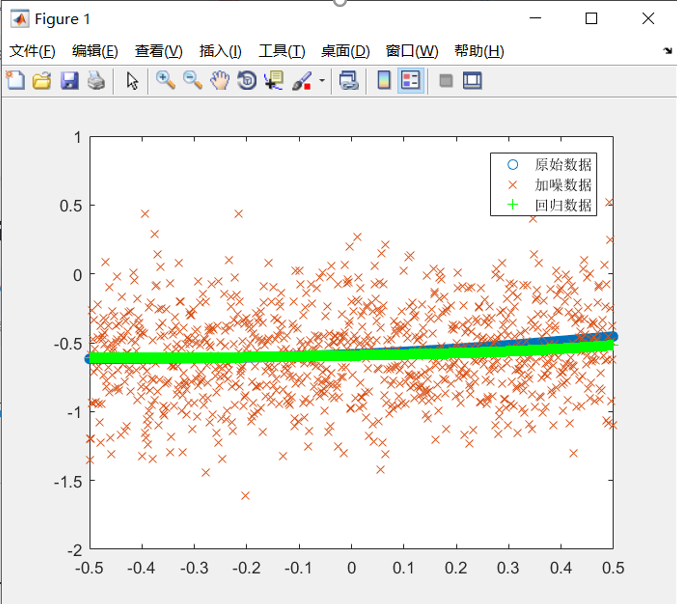
\includegraphics[width=7cm]{pic/res.png}%trim = 0mm 0mm 0mm 0mm,clip,
    \caption{处理结果。}
    \label{fig:res}
\end{figure}


\section{思考与改进}
总的来说本次仿真实验还有很多不足。首先在数据上由于相关知识的缺失,导致退而求其次并没有选择有色噪声而是选择了白噪声。由于MVDR的缺失导致最后在结果上也差强人意
